\documentclass[12pt,a4paper,oneside,parskip=half]{scrreprt}

% Load packages
% Styling
\usepackage[utf8]{luainputenc}
\usepackage[T1]{fontenc}
\usepackage[onehalfspacing]{setspace}
\usepackage[margin=2cm,foot=1cm, includeheadfoot]{geometry}

% Font
\usepackage{palatino}

% Header, Footer, etc.
\usepackage[headsepline]{scrlayer-scrpage}
\pagestyle{scrheadings}
\clearpairofpagestyles

\automark{chapter}
\ihead{}
\chead{}
\ohead{\headmark}
\ifoot{}
\cfoot*{\pagemark}
\ofoot{}

% Images packages
\usepackage{graphicx}
\usepackage{wrapfig}
\usepackage{subcaption}
\usepackage[format=plain, indention=0cm]{caption}

% Links
\usepackage[hidelinks]{hyperref}
\hypersetup{
  linktoc=all
}

% For landscape pages
\usepackage{pdflscape}

% Glossary
\usepackage[toc, nonumberlist, automake, acronyms, nopostdot]{glossaries}

% References
\usepackage{url}
\usepackage[backend=biber, bibencoding=utf8, style=ieee]{biblatex}
\addbibresource{resources/references/ref.bib}

% Math
\usepackage{amsmath}
\usepackage{bm}

% Other
\usepackage{ifthen}    % To switch between the languages
\usepackage{todonotes} % Useful package for notes
\usepackage{multicol}  % 
\usepackage{lipsum}    % Just for the example

% Load the configuration
% Language
\newboolean{german}
\setboolean{german}{false}

% Title Page
\newcommand{\Title}{Project Title}            % Your thesis title
\newcommand{\Author}{Your name}               % Your name
\newcommand{\Projecttype}{Project thesis}     % The type of the thesis 
\newcommand{\Studycourse}{Computer Science}   % Your Course of Study
\newcommand{\Date}{DD.MM.YYYY}                % The Submission date
\newcommand{\Studentnumber}{\dots}            % The editing time 
\newcommand{\Course}{\dots}                   % Your Student number and the designation of your course
\newcommand{\Partner}{\dots}                  % Your company
\newcommand{\Supervisor}{\dots}               % Your company advisor
\newcommand{\Reviewer}{\dots}                 % The reviewer at the DHBW

% Unversity
\ifthenelse{\boolean{german}}{
    \newcommand{\University}{Duale Hochschule Baden-Württemberg Stuttgart}
}{
    \newcommand{\University}{Baden-Wuerttemberg Cooperative State University Stuttgart}
}

% Declaration Page
\newcommand{\DeclarationLocation}{Stuttgart}
\newcommand{\DeclarationDate}{DD.MM.YYYY}


% Language
\ifthenelse{\boolean{german}}{
    \usepackage[ngerman]{babel}
}

% Glossary
\makeglossaries
% Your glossary entries here

% Example
\newglossaryentry{DHBW}{
    name        = {Baden-Württemberg Cooperative State University},
    description = {Baden-Württemberg Cooperative State University is an institution of higher education in Baden-Württemberg}
}
% Acronyms here
\glsaddall

% Roman Numbers
\pagenumbering{roman}

% ----------
% -Document-
% ----------
\begin{document}    

% Cover Page
\begin{titlepage}
    \vspace*{12mm}
	\begin{figure}[th]
        \begin{subfigure}{0.5\textwidth}
            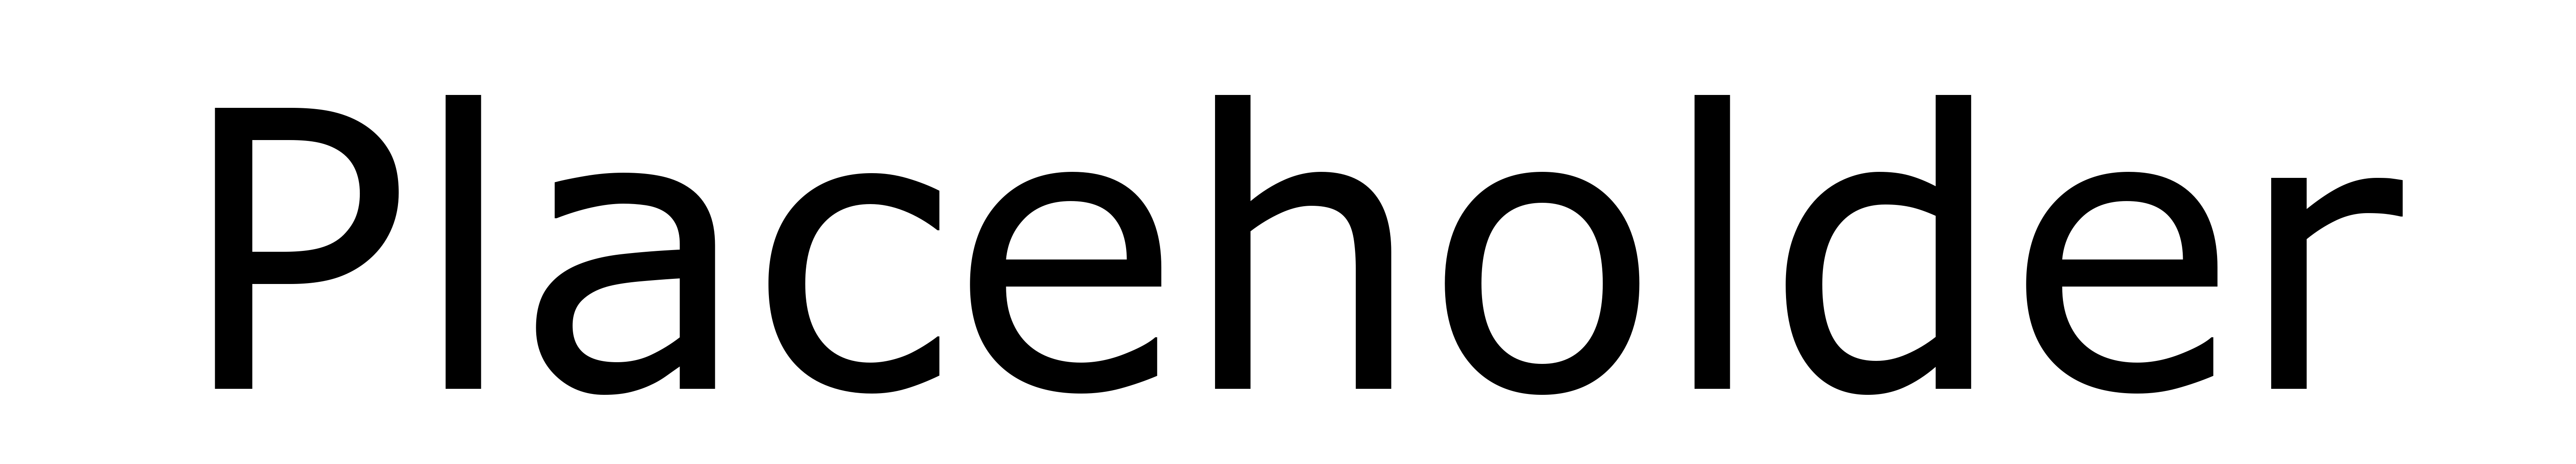
\includegraphics[width=0.8\textwidth]{resources/images/logo/placeholder.png}
        \end{subfigure}
        \begin{subfigure}{0.5\textwidth}
            
\includegraphics[width=0.9\textwidth]{resources/images/logo/DHBW-Logo.png}
        \end{subfigure}
    \end{figure}
    \centering
    \begin{center}
		\vspace*{12mm}	{\LARGE\textbf{\Title} } \\
		\vspace*{12mm}	{\large\textbf{\Projecttype}} \\
		\vspace*{12mm}	\ifthenelse{\boolean{german}}{in dem Studiengang}{of the study program} \\
		\vspace*{3mm}	{\ \textbf{\Studycourse}} \\
		\vspace*{12mm}	\ifthenelse{\boolean{german}}{an der}{at the} \\
        \vspace*{3mm}	{\textbf{\University}} \\
		\vspace*{12mm}	\ifthenelse{\boolean{german}}{von}{from} \\
		\vspace*{3mm}	{\large\textbf{\Author}} \\
		\vspace*{12mm}	\Date \\
	\end{center}
    \vspace*{6mm}
    \begin{tabular}{l l}
        \ifthenelse{\boolean{german}}{Matrikelnummer}{Studentnumber} & \Studentnumber \\
        \ifthenelse{\boolean{german}}{Kurs}{Course} & \Course \\
        \ifthenelse{\boolean{german}}{Dualer Partner}{Dual partner} & \Partner \\
        \ifthenelse{\boolean{german}}{Betreuer:in des Dualen Partners}{Supervisor of the dual partner} & \Supervisor \\
        \ifthenelse{\boolean{german}}{Gutachter:in der DHBW}{Reviewer of the Dual University} & \Reviewer
    \end{tabular}
\end{titlepage}
\newpage

% Declaration
\ifthenelse{\boolean{german}}{
    \chapter*{Erklärung}
    Ich versichere hiermit, dass ich meine Bachelorarbeit (bzw. Projektarbeit oder Studienarbeit bzw. Hausarbeit) mit dem Thema \textbf{\Title}  selbstständig verfasst und keine anderen als die angegebenen Quellen und Hilfsmittel benutzt habe. Ich versichere zudem, dass die eingereichte elektronische Fassung mit der gedruckten Fassung übereinstimmt.
}{
    \chapter*{Declaration}
    I hereby certify that I have written my project work with the topic: \textbf{\Title} independently and have not used any sources and aids other than those indicated. I also assure that the submitted electronic version corresponds to the printed version.

}

\vspace{4em}

\DeclarationLocation, \DeclarationDate

\vspace{3em}

\rule{6cm}{0.4pt}\\
\newpage

% Confidentiality
\ifthenelse{\boolean{confidential}}{
    \ifthenelse{\boolean{german}}{
        \chapter*{Vertraulichkeit}
        Der Inhalt dieser Arbeit darf weder als Ganzes noch in Auszügen Personen außerhalb des Prüfungsprozesses und des Evaluationsverfahrens zugänglich gemacht werden, sofern keine anders lautende Genehmigung des Dualen Partners vorliegt.
    }{
        \chapter*{Confidentiality}
        The contents of this thesis may not be made available, either in whole or in excerpts, to persons outside the review process and the evaluation process, unless otherwise authorized by the Dual Partner.
    }
    \newpage
}{}

% Abstracts
\chapter*{Abstract}

% TOC
\tableofcontents
\newpage

% List of Figures
\addcontentsline{toc}{chapter}{\listfigurename}
\listoffigures
\newpage

% List of tables
\addcontentsline{toc}{chapter}{\listtablename}
\listoftables
\newpage

% Acronyms
\ifthenelse{\boolean{german}}{
    \printglossary[type=\acronymtype, title=Akronyme]
}{
    \printglossary[type=\acronymtype]
}

% =============================
% == Place your content here ==

% Example of how .tex files can be inserted (Can be removed) 
\chapter{Wikipedia is not a reliable source}

% Set "page numbering" to arabic after the first chapter heading
\pagenumbering{arabic}

\lipsum[1]
\cite{wiki:lorem_ipsum}

% =============================

% References
\printbibliography
\newpage

% Glossary
\printglossary
\glsaddallunused % Print all Glossary entries

\end{document}